\graphicspath{{chapters/ThebasicsImages/}}


\chapter{Introduction}

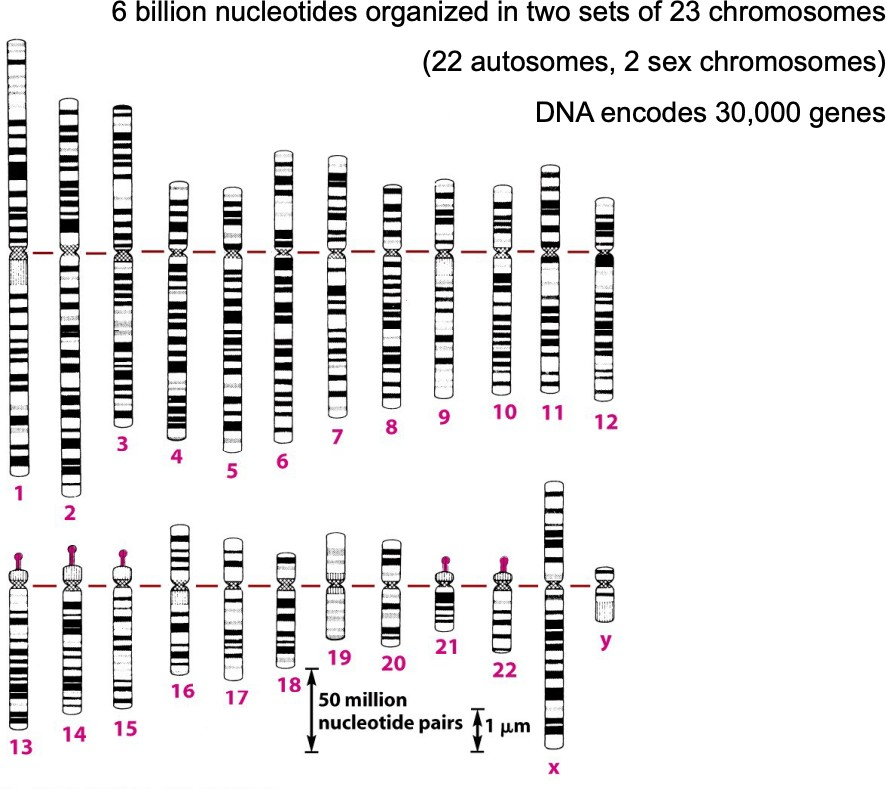
\includegraphics[width=4.32507in,height=3.86281in]{image1.jpeg}

\begin{quote}
The words variations, aberrations and lesions are often interchanged.
Aberrations and lesions are mainly used for acquired lesions, instead
variations are mainly used for the inherited ones.
\end{quote}

\hypertarget{genetic-make-up}{%
\subsection{Genetic Make-Up}\label{genetic-make-up}}

\begin{quote}
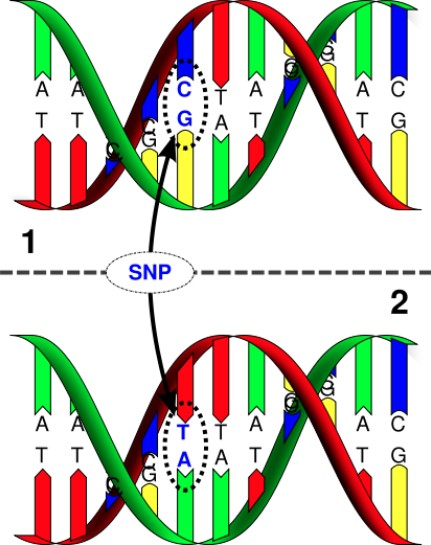
\includegraphics[width=1.97816in,height=2.50248in]{image2.jpeg}A
\textbf{Single Nucleotide Polymorphism} (SNP) is a sequence variation
affecting single amino acid → point mutation.

The genomes of two unrelated individuals have about 1\% of different
bases → that percentage corresponds to the SNPs.

But looking at the \textbf{Copy Number}

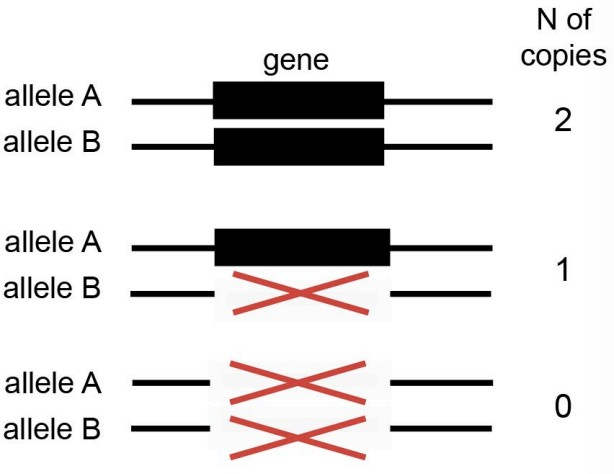
\includegraphics[width=2.93475in,height=2.26167in]{image3.jpeg}\textbf{Variants}
(CNV), that difference will be way higher than only 1\%

DNA not present in only two copies, but in multiple, single or even zero
copies (hemizygous loss, homozygous loss)

They are less known as inherited type of variants because they are
harder to detect and identify, but they provide a lot of uniqueness in
each of us.

Why are SNPs and CNVs so important?

They are responsible of human diversity → genetic changes

Hundreds of CNVs per individual and 20\% of them potentially affect
protein- coding genes

\textbf{Differences} in Genetic Make-up:

Very common variants are variants that are distributed in the population
as the common allele, so that 1/2 of the population has an heterozygous
genotype at that position, 1/4 has an homozygous genotype for one allele
and 1/4 has an homozygous genotype for the other allele.

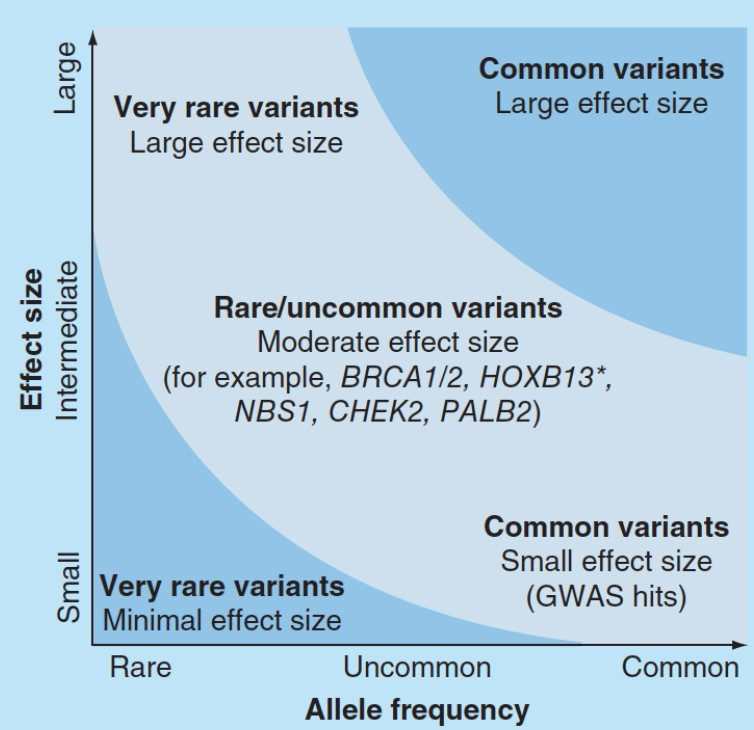
\includegraphics[width=3.9928in,height=3.87812in]{image4.jpeg}

The \textbf{penetrance} is the proportion of individuals carrying an
allele (or a genotype) that also expresses the trait (phenotype)
associated with it. Obviously, penetrance is directly associated with
the size of the effect produced by the variant.

The \textbf{allele frequency} is calculated by dividing the number of
times the allele of interest is observed in a population by the total
number of copies of all the alleles at that particular genetic locus in
the population.

The allele frequency is low with very rare variants

Well known variants: BRCA1/2, HOXB13, NBS1, PALB2, CHEK2 → they have
moderate size effects, meaning that all the people who have the
variants, have the disease
\end{quote}

\hypertarget{differences-in-genetic-make-up-example}{%
\subsubsection{Differences in genetic Make-Up,
example}\label{differences-in-genetic-make-up-example}}

\begin{quote}
Absorption, distribution, metabolism and elimination (ADME) genetic
variants determine pharmacokinetic variability of certain compounds,
influencing the patients' treatment response. Both common and rare
variants are involved.

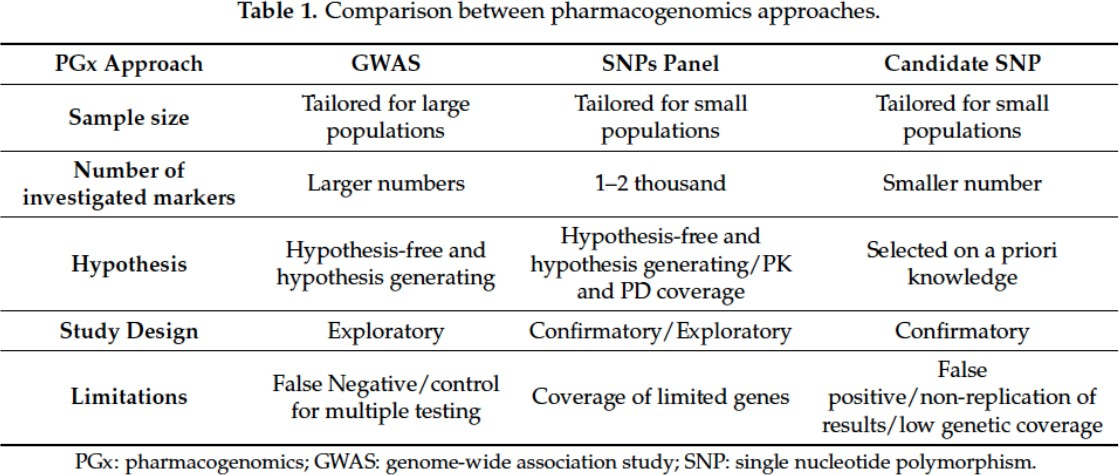
\includegraphics[width=6.18852in,height=2.6224in]{image5.jpeg}

Three main ways to study genetic variants: GWAS (genome-wide association
study)

SNPs panel Candidate SNP

For example, in terms of hypothesis, if I study all the variants in the
human genome and I query them in a large population, I generate data
without specifying SNP to search. Instead, if I have a very specific
hypothesis, for example I want to query if a SNPs in the CYP gene
relates to the conversion of androgens to estrogens, I don't need to run
an GWAS or a wide SNPs panel. I can query those SNPs because I have an
\emph{a priori} hypothesis and I want to test them.

This type of differential design for an experiment it is not only true
for inherited variants and ADME genes, but also to predisposition to
diseases and to study human tumors.

Precision medicine → treatment (or dosage) of a patient based on their
individual traits: takes into consideration genetic and genomic of the
individual and tumor/disease cells

Starch rich diet → CNV in the genome Drink beer and turn red → ADME gene

Athletes with a deletion of a gene, the steroids were not found in the
anti-doping tests
\end{quote}

\hypertarget{acquired-dna-aberrations}{%
\subsection{Acquired DNA aberrations}\label{acquired-dna-aberrations}}

\begin{quote}
Somatic variants are the variants NOT inherited from parents and not
transmitted to offspring. They are:

\textbf{Single Nucleotide Variants} (SNV) are somatic changes of single
nucleotides present in only certain cells, instead of SNPs that are
present in all cells of our body.

\textbf{Indels} are changes that involve few nucleotides by INsertion
and DEletion

\textbf{Rearrangements} are mutations that can involve events like
translocations, inversion, chromothripsis,.. usually these events are
caused by breakage in the DNA double helices a two different locations,
followed by a rejoining of the broken ends to produce a new chromosomal
arrangement of genes, different from the beginning

\textbf{Somatic copy number aberrations} (\textbf{SCNA}) are somatic
changes similar to CNVs. They can be every change related to the number
of copies like loss of a portion of a genome, loss of both alleles,
extra copies...

\textbf{Examples} of acquired DNA aberrations:
\end{quote}

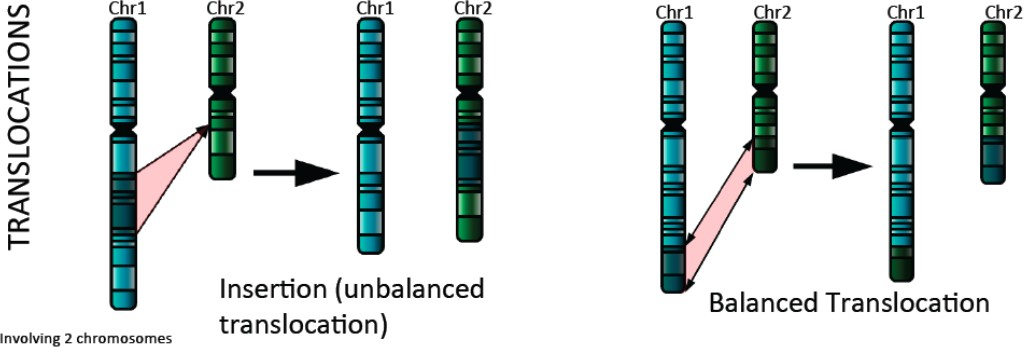
\includegraphics[width=6.1748in,height=2.09646in]{image6.jpeg}

\begin{quote}
\textbf{Balanced translocation}: you conserve the quantity of DNA, there
isn't any loss or gain

\textbf{Unbalanced translocation}: A genomic portion is translocated
from a chromosome to another, there is not vice versa.

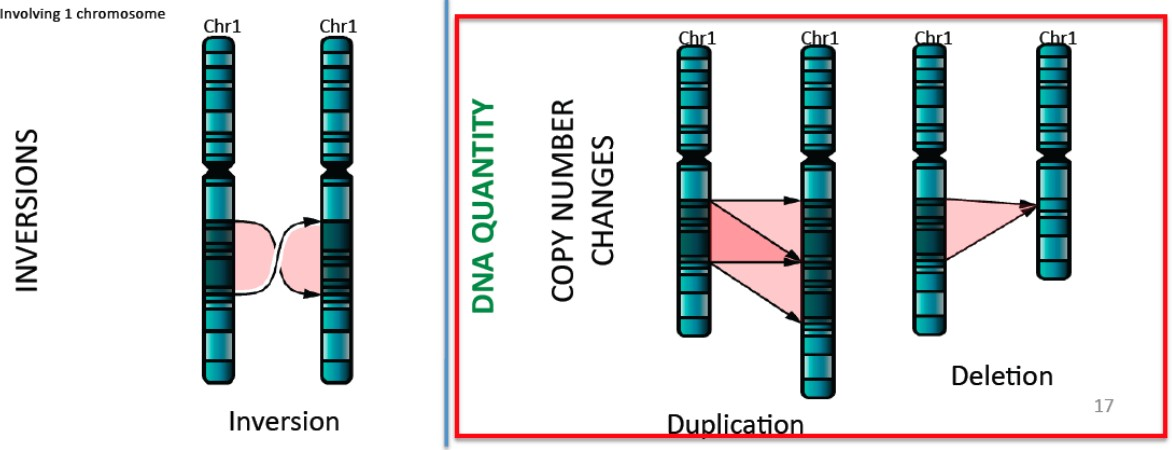
\includegraphics[width=6.22722in,height=2.39062in]{image7.jpeg}

\textbf{Inversions} in only ONE chromosome: everything is normal instead
in the break points

\textbf{Copy number changes:} duplication or deletion

It could happen in the same chromosome but also in different chromosomes

Other types of complex somatic events include:

\textbf{Chromoplexy}: a class of complex somatic DNA rearrangements
whereby abundant DNA deletions and intra- and inter-chromosomal
translocations that have originated in an interdependent way occur
within a single cell cycle

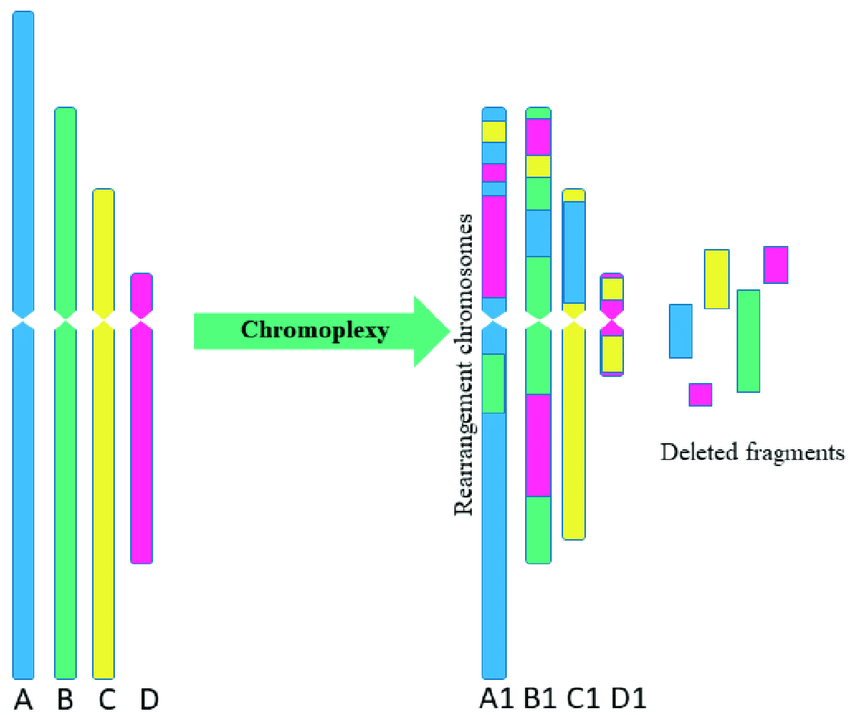
\includegraphics[width=3.81944in,height=3.21433in]{image8.png}

\textbf{Chromothripsis}: a clustered chromosomal rearrangement in
confined genomic regions that results from a single catastrophic event,
usually limited to one chromosome

\textbf{Kataegis}: a phenomenon that is characterized by large cluster
of mutations (hypermutation) in the genome of cancer cells. An APOBEC
family enzyme might be responsible fo the kataegis process


when an aberration (clonal) occurs, all the cells will harbour the
aberration and at some point another aberration (subclonal of the other)
could appear in just one cell line. The \textbf{clonal} aberration is
present in all the cells, the \textbf{subclonal} aberration is inherited
in just one cell line. Clonality is an important information that allow
us to study evolution.
\end{quote}

\hypertarget{experimental-approaches}{%
\section{Experimental approaches}\label{experimental-approaches}}

\begin{quote}
Experimental techniques to detect variants/aberrations \textbf{prior to
NGS}: a failure because it was very hard to determine the starting
points of the aberrations
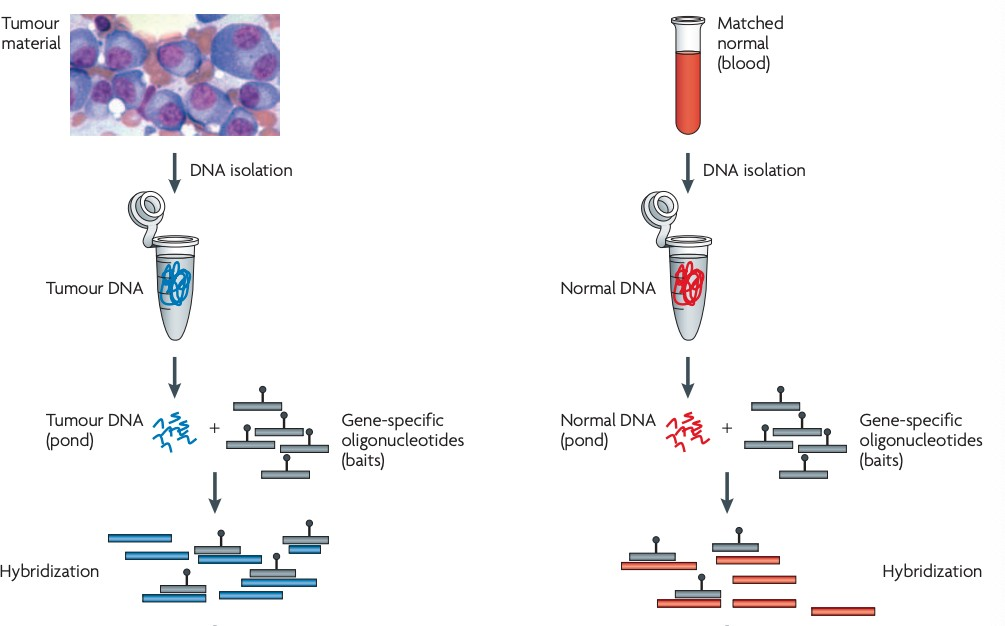
\includegraphics[width=6.18343in,height=3.84729in]{image9.jpeg}(Meyerson
et al. 2010, ``Advances in Understanding Cancer Genomes through
Second-Generation Sequencing.'', Nature Reviews Genetics,
\url{https://doi.org/10.1038/nrg2841}).

Bulk of tumor tissue/cells from the blood:
\end{quote}

\begin{enumerate}
\def\labelenumi{\arabic{enumi})}
\item
  DNA isolation
\item
  Gene-specific oligonucleotides (\textbf{baits}) that get hybridized
  onto the tumor DNA → the baits have a tag that allows them to be
  isolated
\item
  The DNA does get fragmented
\item
  The captured DNA is eluted and prepared into sequencing libraries
\item
  Sequenced
\item
  Aligned to the bait sequences
\end{enumerate}

\begin{quote}
We repeat the procedure for healthy cells of the same individual in
order to \textbf{detect somatic mutations} and distinguish them from the
germline (= match normal)
\end{quote}

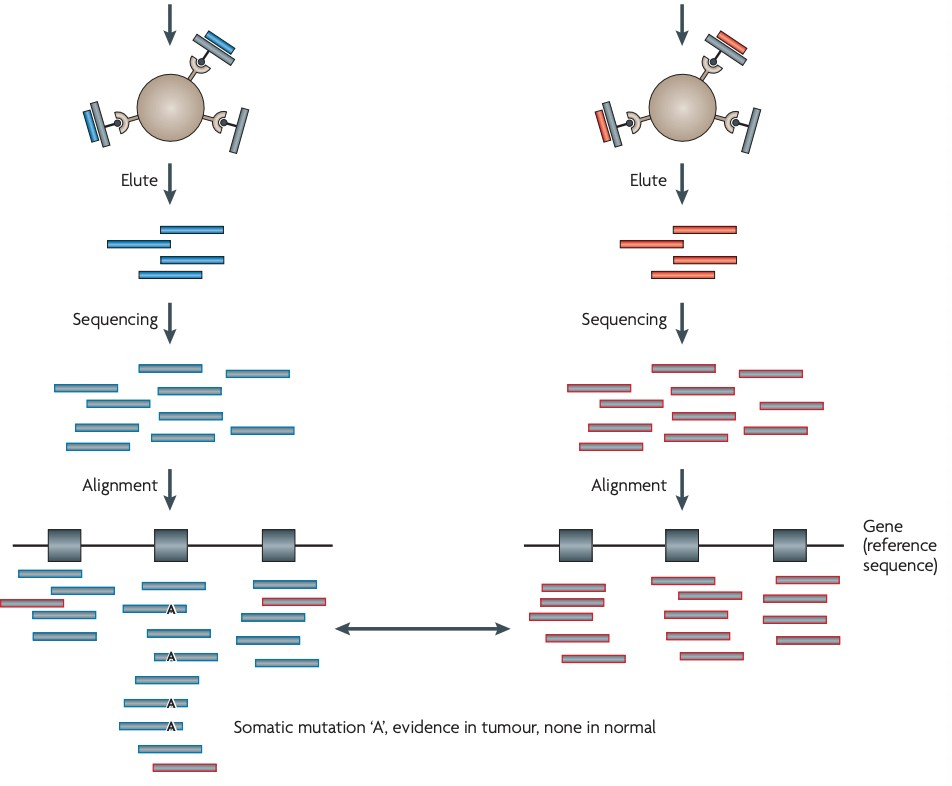
\includegraphics[width=6.14828in,height=5.07625in]{image10.jpeg}

\begin{quote}
We sequence baits because is way cheaper (exons of 50 bases instead the
whole genome)

After fragmentation procedure, before adding the adapters, we can choose
between two different sequencing approaches:
\end{quote}

\hypertarget{single-end-se-sequencing}{%
\subsubsection{Single End (SE)
sequencing}\label{single-end-se-sequencing}}

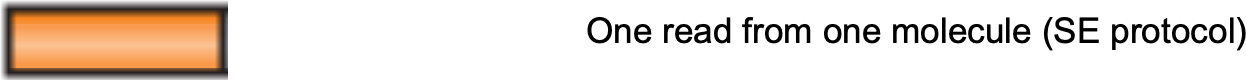
\includegraphics[width=5.64649in,height=0.35833in]{image11.png}

\begin{quote}
You will sequence only one part of a molecule (length of 150 bp
→ based on the power of the sequencing machine we are using). You will
know exactly 150 bp for every molecule you sequence, but you lose
information (the second end of the pair)
\end{quote}

\hypertarget{paired-end-pe-sequencing}{%
\subsubsection{Paired End (PE)
sequencing}\label{paired-end-pe-sequencing}}

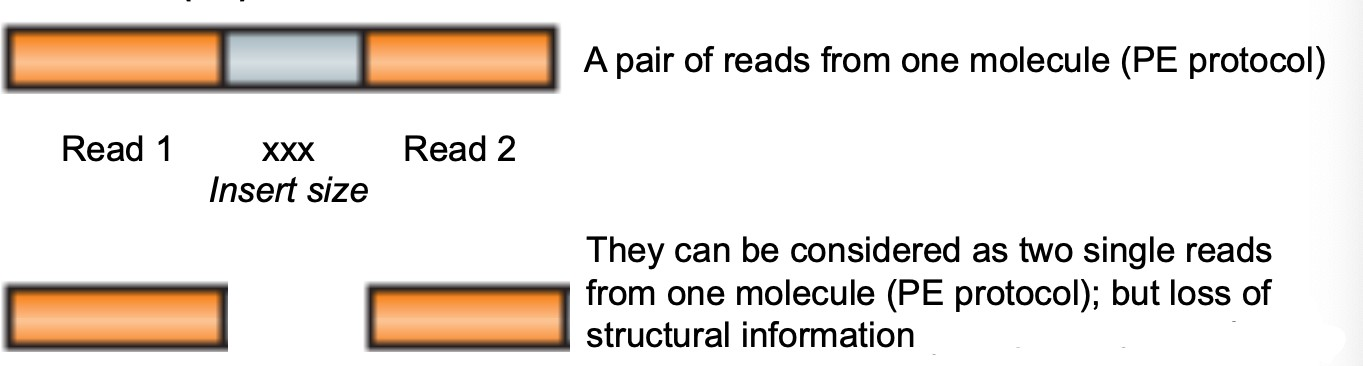
\includegraphics[width=5.97751in,height=1.60125in]{image12.jpeg}

\begin{quote}
This method lose only the information between the two ends (= insert
size) but you will know the exact length of the entire molecule. You can
compare the \textbf{expected} insert size with what it has been
generated.

It's more expensive, but:
\end{quote}

\begin{itemize}
\item
  it gives information about the localization of the molecule
\item
  you can treat each end as single read
\end{itemize}

\begin{quote}
In the following picture: a view of reads that are mapped against
reference genome and what we would look if we have any of the variations
that we mentioned
\end{quote}

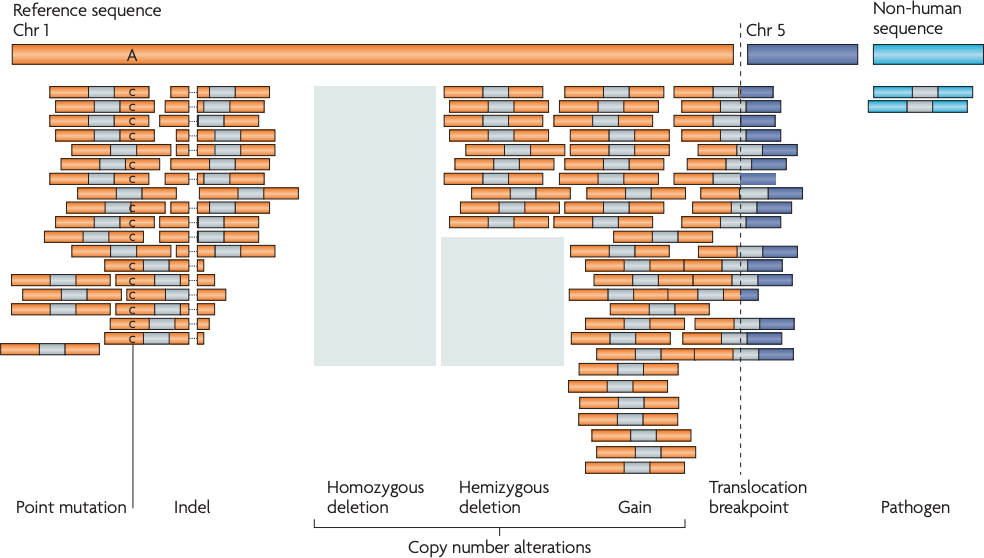
\includegraphics[width=6.16003in,height=3.4875in]{image13.png}

\begin{quote}
Different types of genomic alteration can be detected:

You can clearly identify \textbf{point mutations}. If a point mutation
is present in the molecule that you sequenced and present on both
alleles of the genome, it can be seen in all the reads very clearly

You might see \textbf{indels} (shown here by a dashed line). You will
see a little space because the reference genome has more nucleotides
than the sequenced molecule

If you have \textbf{homozygous deletion}, you don't see anything mapped
in that portion: there's no DNA. Doesn't matter if SE or PE.

If you have \textbf{hemizygous deletion}, you see the see the read
mapped to that portion where the hemizygous deletion is sitting, that is
more or less proportional to half of the reads that you have in regions
where you don't have a copy number change. Doesn't matter if SE or PE

If you have \textbf{gain}, what you get is higher number of reads
aligned against that part of DNA, underlying the fact that the molecule
you sequenced has extra DNA for that portion of reference genome.
Doesn't matter if SE or PE

\textbf{Translocation breakpoint} are very important!! You will have one
end mapping the chr1 and the other end mapping the chr5. Those two ends
come from the same molecule of the \emph{target cell} (the cell we
sequenced), it means the cell has a translocation between chr1 and chr5.
Without the PE protocol you cannot have this result
\end{quote}

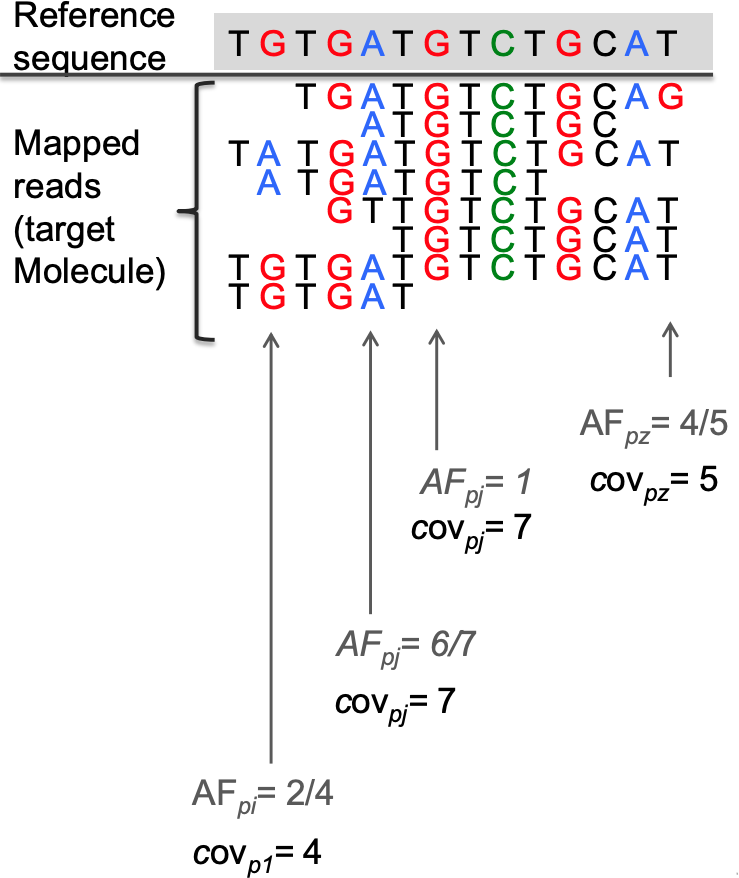
\includegraphics[width=3.00163in,height=3.56687in]{image14.png}

\begin{quote}
The \textbf{local coverage} (cov) at position \emph{i} is the number of
reads that span \emph{p\textsubscript{i}}

The \textbf{allelic fraction} (AF) at position \emph{i} is the
proportion of reads that supports the reference base in
\emph{p\textsubscript{i}} (= the reference or the alternative allele)

\textbf{Whole Genome Sequencing Coverage}

% \emph{L} ⋅ \emph{N}

\emph{cov} =

\emph{G}

where:
\end{quote}

\begin{itemize}
\item
  L is the read length
\item
  N is the number of mapped reads
\item
  G is the haploid human genome length
\end{itemize}

\begin{quote}
This is super important because it saves us time and money when we
design an experiment. When you design an NGS experiment, you should know
up front what is the type of coverage you need to answer the question
you wanna ask with your experiment. For example, if you want to look at
the genotype of SNPs (inherited polymorphisms at single side), you don't
really need a coverage which is above 10 or 15. So you can design your
experiment in order to have an average coverage equal to 10 or 15. To do
that, you reverse the equation and count how many reads you need to
generate to achieve that goal.

N.B. The number of mapped reads will be always lower of the number of
reads generated by the machine (than the expected). There might be
duplicates that you might not be able to use because there might be
reads that have a quality below the threshold you intend to use
\end{quote}

\hypertarget{difference-between-sequence-coverage-and-physical-coverage}{%
\subsubsection{Difference between sequence coverage and physical
coverage}\label{difference-between-sequence-coverage-and-physical-coverage}}

\begin{quote}
A graphic view of how SE or PE can be used:
\end{quote}

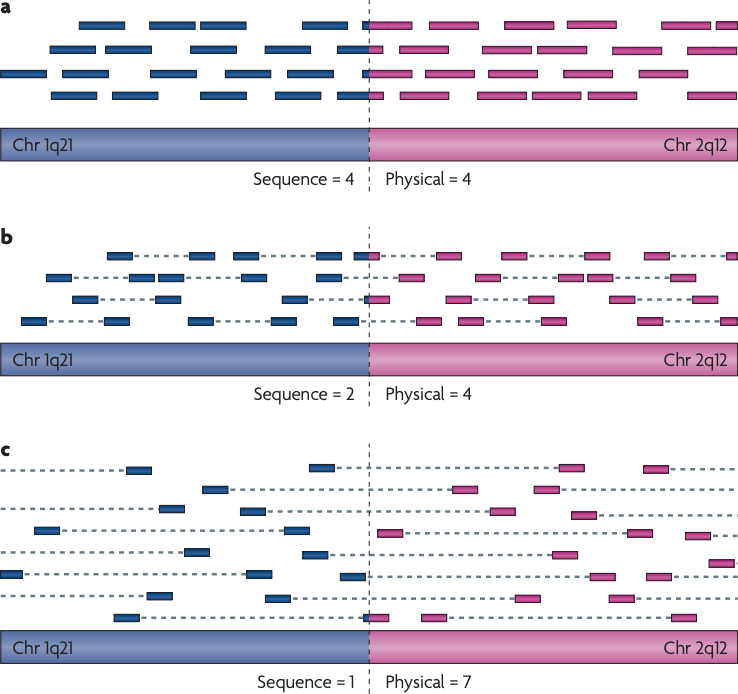
\includegraphics[width=5.99692in,height=5.63875in]{image15.png}

\begin{quote}
Panel A - SE protocol Panel B - PE protocol Panel C - PE protocol

Three different scenario are depicted that vary in the length of the DNA
fragments that are sequenced. \textbf{Sequence coverage} represents the
number of sequenced reads that cover the site; this affects the ability
to detect point mutations. \textbf{Physical coverage} measures the
number of fragments that span the site; this affects the ability to
detect the rearrangement, based on paired reads that map to different
chromosomes. It is a way informative type of coverage: for instance for
translocations, deletions,..

In Paired End sequencing protocols, the physical coverage is always
higher than the sequence coverage because it takes into consideration
also the insert sizes

Making estimation of intended coverage and observed coverage is very
important. Here are few examples:

In these panels were designed to sequence a set of 10 genes that the
researchers were interested in for prostate cancer. They designed this
panel, sequenced cell lines on this panel and observed the following
points

On x-axis: the genomic location

On y-axis: the local coverage (amplicon median coverage = each bar
represents the local coverage of about 30 bp)

The different colors represent the different genes
\end{quote}

\hypertarget{st-panel---lncap-sample-cell-line}{%
\subsubsection{1st panel - LNCaP sample (cell
line)}\label{st-panel---lncap-sample-cell-line}}

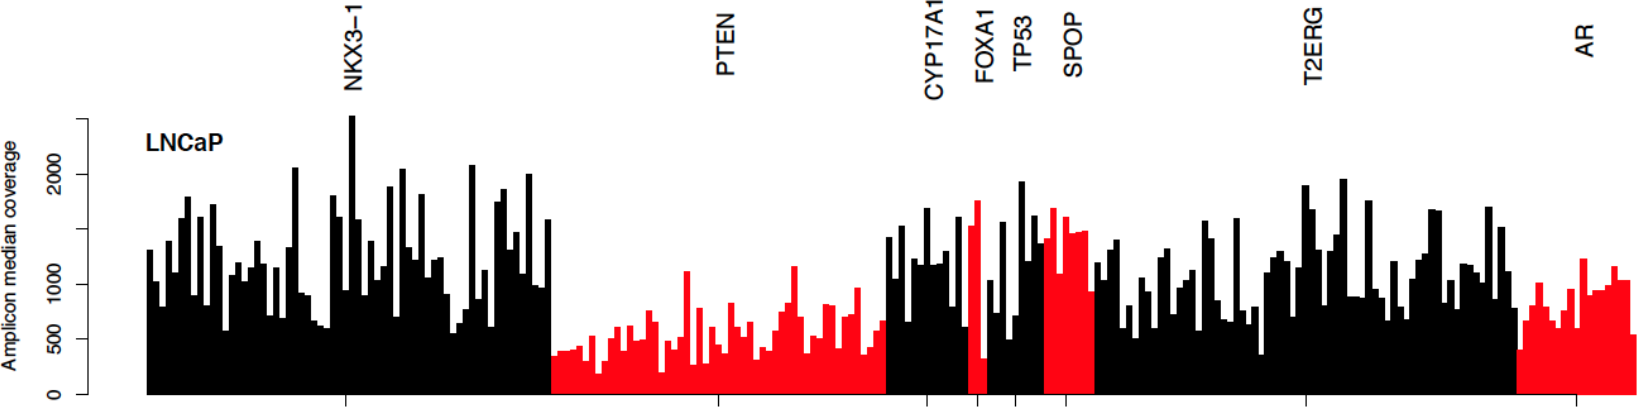
\includegraphics[width=6.13481in,height=1.52625in]{image16.png}

\begin{quote}
Local coverage (pile-up) of selected areas (targeted sequencing assay):
7 genes

+ 1 multi-gene region (T2ERG). Alternate colors indicate targeted areas
The barplot show a single sample (LnCaP cell line; cancer cell line)
data.

Apparent \textbf{deletion} of PTEN (monoallelic deletion) because the
local coverage of PTEN is significantly lower than the one from other
genes.
\end{quote}

\hypertarget{nd-panel---pc3-sample-cell-line}{%
\subsubsection{2nd panel - PC3 sample (cell
line)}\label{nd-panel---pc3-sample-cell-line}}

\begin{quote}
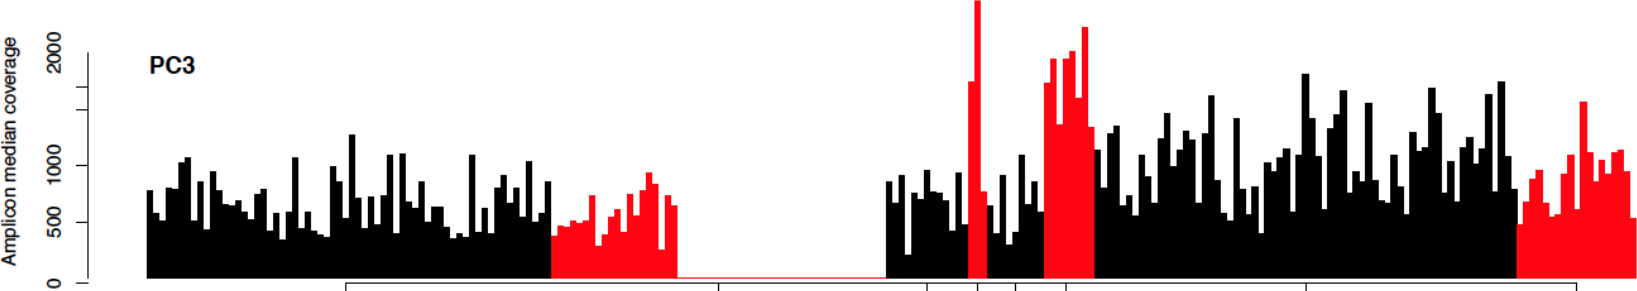
\includegraphics[width=6.15327in,height=1.09125in]{image17.png}

Local coverage (pile-up) of selected areas (targeted sequencing assay):
7 genes

+ 1 multi-gene region.

Monoallelic deletion and partial biallelic deletion of PTEN because one
portion is deleted and one not. PTEN has a \textbf{partial homozygous
deletion}.

The PC3 cell line shows a little bit of gain in the gene SPOP and FOXA1.

The average coverage for the PC3 cells is approximately the same as the
previous sample.
\end{quote}

\hypertarget{rd-panel---vcap-sample-cell-line}{%
\subsubsection{3rd panel - VCaP sample (cell
line)}\label{rd-panel---vcap-sample-cell-line}}

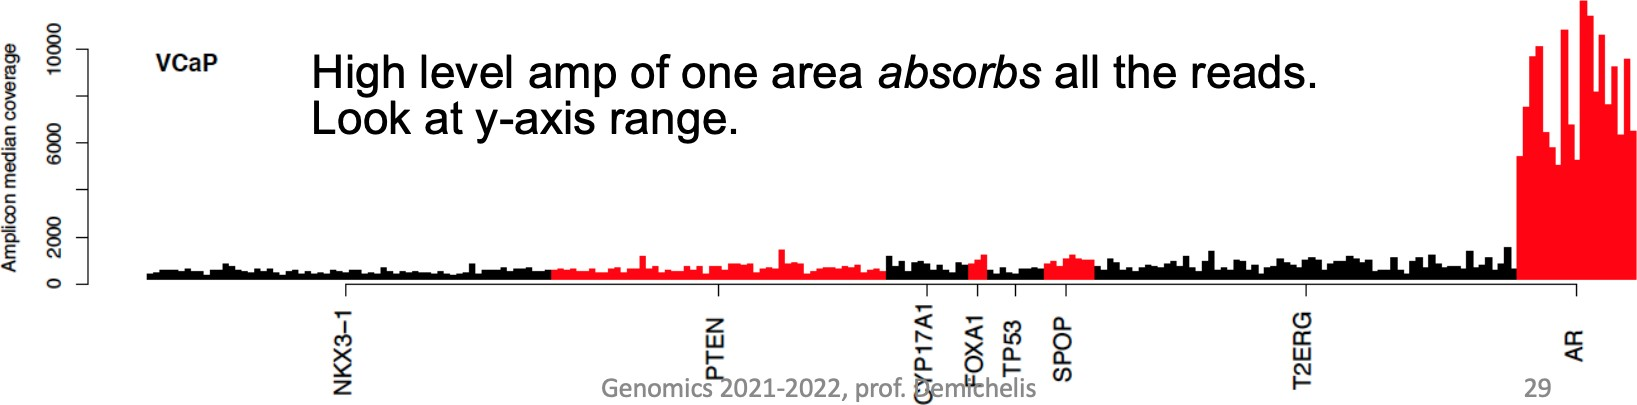
\includegraphics[width=6.17134in,height=1.51875in]{image18.jpeg}

\begin{quote}
There's no homozygous deletion but has a high level amplification of one
area \emph{absorbs} all the reads. Massive amplification of the Androgen
Receptor (AR) → error: because it inhibits the sensitivity of detecting
copy number changes in any other gene.

When designing a panel we must pay attention and make sure that we don't
have potential aberration that basically will draw all the attention of
your experiment and leave you without information or sensitivity in all
other regions.

It's easy to increase the experimental coverage (i.e. the sequence
depth) at later point. Provided tour original sample/library is still
available, you can perform another run of sequencing and then combine
the output from different runs
\end{quote}

\hypertarget{note-that-this-isnt-possible-with-array-based-technologies.}{%
\subsubsection{Note that this isn't possible with array-based
technologies.}\label{note-that-this-isnt-possible-with-array-based-technologies.}}

\begin{quote}
What are the limiting factors of NGS DNA-seq experiment, in any?

Repeated regions due to \textbf{short reads}

What is the problem of short sequencing on long genome?

Complexity regions CG content
\end{quote}

\hypertarget{the-reference-sequence-of-the-human-genome}{%
\section{The reference sequence of the human
genome}\label{the-reference-sequence-of-the-human-genome}}

\begin{quote}
Many years ago, some people claimed that the entire human genome was
sequenced but it wasn't true at all. There were still unknown or missing
regions. In 2022 we finally have the complete human reference genome
sequence.

But we need to consider the polymorphisms, there is no \textbf{unique}
genome. How to integrate them into a single reference genome? There is a
consortium that deals with these problems. They assemble a reference
genome that reflects the more common (in the whole population) sequences
at each position of the human genome, but also tracks information of
everything that is polymorphic. So that we can use the latest release of
what they built as reference genome and then use databases to learn
about all the polymorphic sites and all the features of every
polymorphic variants

Genome Reference Consortium:
% \href{https://www.ncbi.nlm.nih.gov/grc/human}{\uline{htt}p\uline{s://www.ncbi.nlm.nih.gov/grc/human}}
where you can find different versions of human reference genome

UCSC Genome Browser on Human:
% \href{http://genome-euro.ucsc.edu/}{\uline{htt}p\uline{://genome-euro.ucsc.edu/}}

where you can upload different versions of the reference
\end{quote}

\hypertarget{interpreting-pair-orientation}{%
\subsection{Interpreting pair
orientation}\label{interpreting-pair-orientation}}

\begin{quote}
Using IGV (Integrative Genomics Viewer)

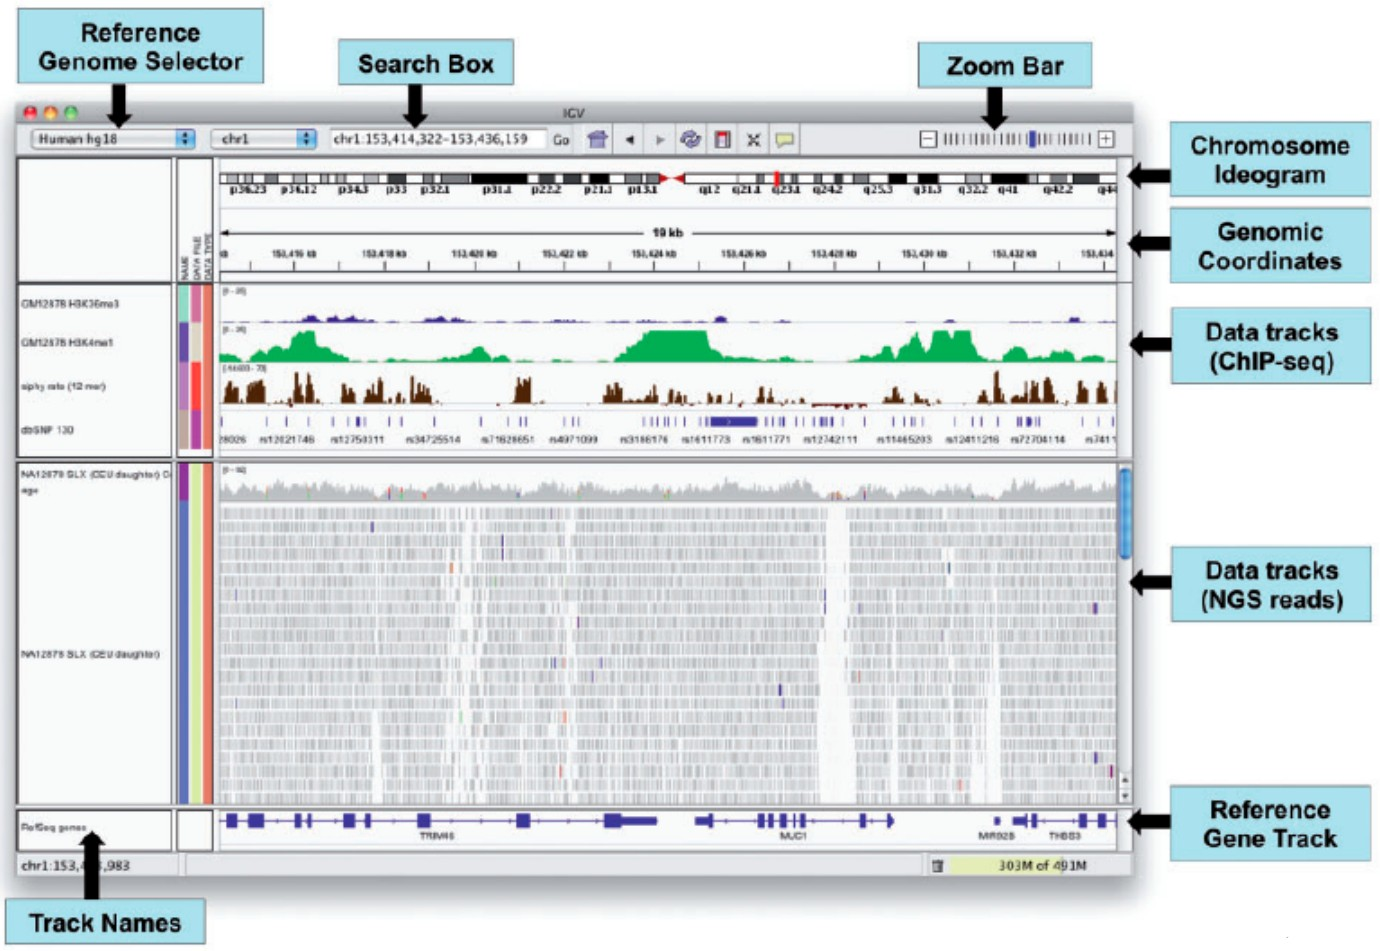
\includegraphics[width=6.32631in,height=4.35875in]{image19.jpeg}

The main characteristic of IGV is that it is a main view viewer: all the
information are in one window

Every vertical bar is a read

On the x-axis there's the genome coordinates at the top, the reference
genome at the bottom (we can select the reference genome we prefer)

Along with the data tracks there is the local coverage of the kb shown
in the window (of the sample we are looking at)

You can get any information you want of any single read that you are
uploading, very useful to see difference from the reference genome
because every aberration or whatsoever is highlighted by a different
color in the local coverage of a nucleotide base. Moreover, it gives
information about the quality of the read and the bases, if you have a
PE protocol, it tells you also information about the PE for each of them

The \textbf{orientation} of paired end can be used to detect structural
events, including: inversions

duplications translocations

According to the Illumina protocol, the two ends are LR oriented, but we
could also obtain other orientations, like LL RR RL, if we come up
against the events mentioned above.
\end{quote}

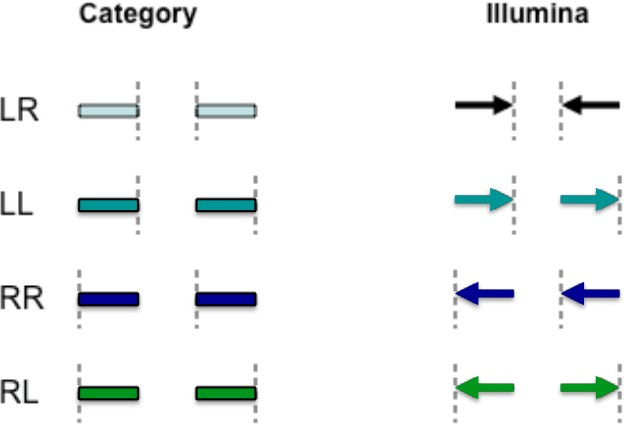
\includegraphics[width=3.89062in,height=2.65in]{image20.jpeg}

\begin{quote}
LR normal reads. They are left and right (respectively) of the
unsequenced part of the sequenced DNA fragment when aligned back to the
reference genome

LL, RR implies inversion in sequenced DNA with respect to reference RL
implies duplication or translocation with respect to reference
\end{quote}

\hypertarget{inversion}{%
\subsection{Inversion}\label{inversion}}

\begin{quote}
A segment of DNA is inverted
\end{quote}

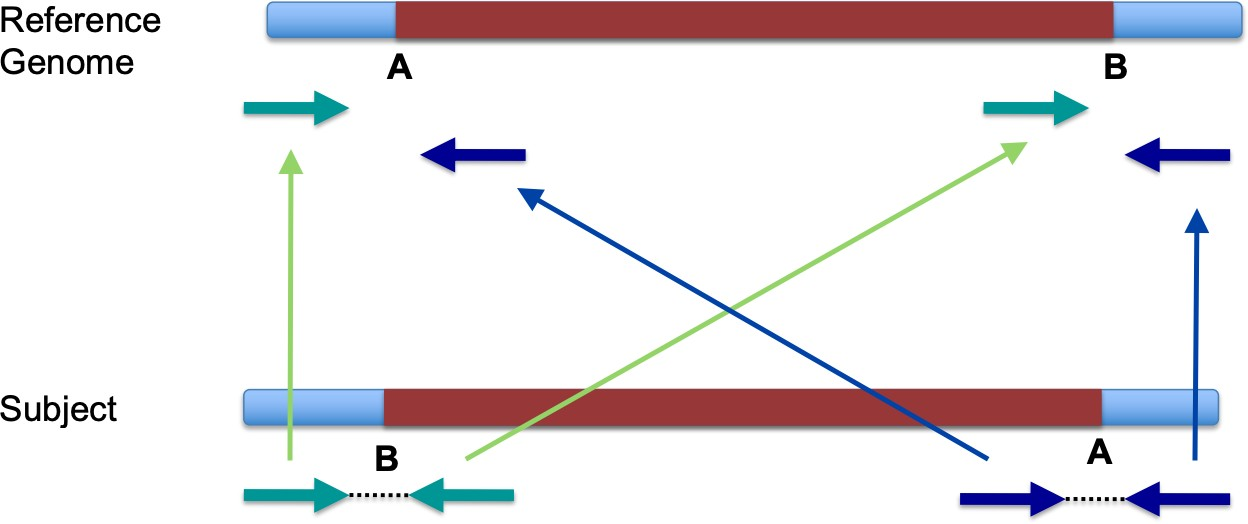
\includegraphics[width=5.85745in,height=2.45625in]{image21.jpeg}

\begin{quote}
The most important pairs are the ones that stand between junctions
because they are the most informative ones.

Here one end mapped where it was on the reference genome while the other
end reversed its orientation

In IGV:
\end{quote}

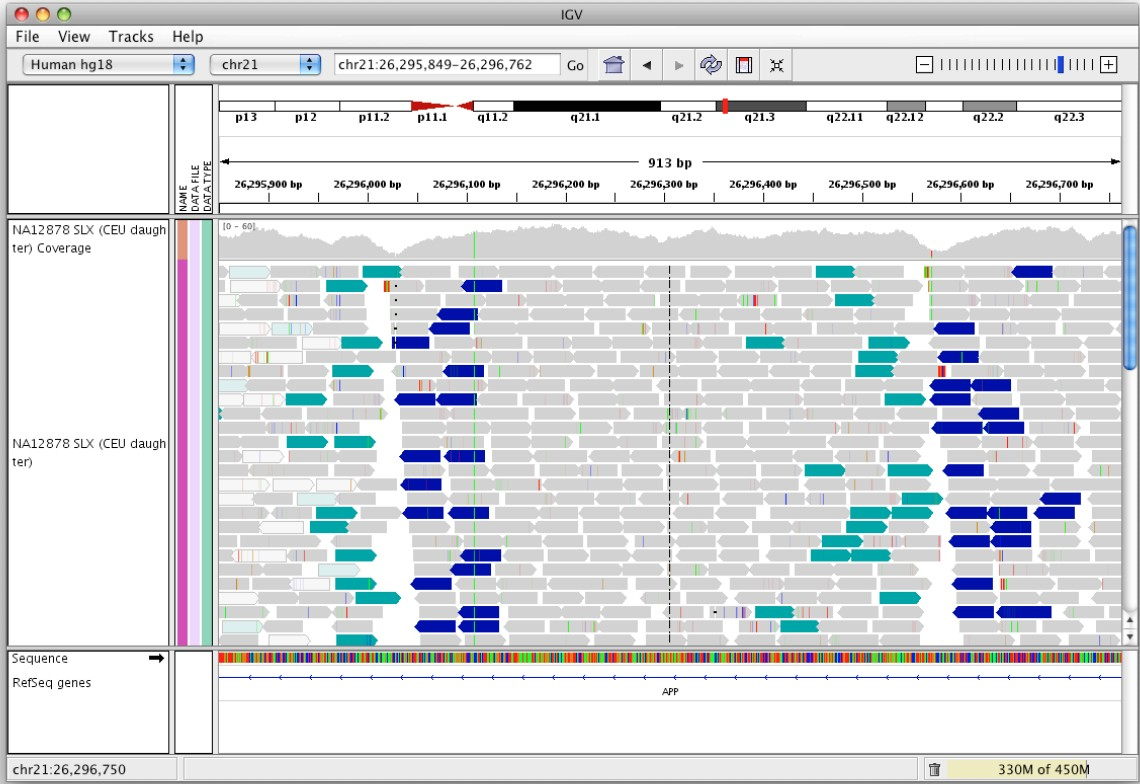
\includegraphics[width=6.29861in,height=4.32833in]{image22.jpeg}

\begin{quote}
Information that help us:

The insert size from the target molecule (= the subject) is way longer.
For all the pairs that are at the breakpoint, the insert size is
different from the expected

The orientation is different

If you look at the local coverage, you can see a \textbf{drop} in two
points: at the breakpoints. The reads that are mapping the junctions
cannot map the reference genome because the breakpoint sequence does not
exist in the reference genome. So, if we have an inversion in only one
of the two alleles, then the reads coming from the allele with the
inversion will not contribute to the local coverage at the breakpoint.
The sequence in your target molecule exists only in one allele, so at
the breakpoints you will only have reads contributing to the local
coverage coming from one allele. The allele with the inversion will not
have the

AB sequence, but only the BA sequence. That's the why of the drop in the
local coverage.

Moreover, we can notice that the coverage on the middle part does not
change significantly from the coverage on the sides. That suggest this
is not either a gain or a deletion, the only thing that might have
happened is an inversion. Therefore, the inversion is not biallelic
(because we see DNA, the drop doesn't go to 0)

When you align reads against a genome, you can allow for a certain
mismatches or partial alignment. So, if you impose certain thresholds to
your aligner, you can also say that if there are reads that align for
80\% and have 20\% of sequences misaligned, you align them in any case.
So you will have reads that are correct up to the breakpoints and the
browser will shows the mismatches beyond the breakpoint. So, you can
have a partial drop of coverage because you allow mismatches in your
alignment.
\end{quote}

\hypertarget{tandem-duplication}{%
\subsection{Tandem duplication}\label{tandem-duplication}}

\begin{quote}
A segment of DNA is duplicated and inserted in the target molecule
adjacent to the original one
\end{quote}

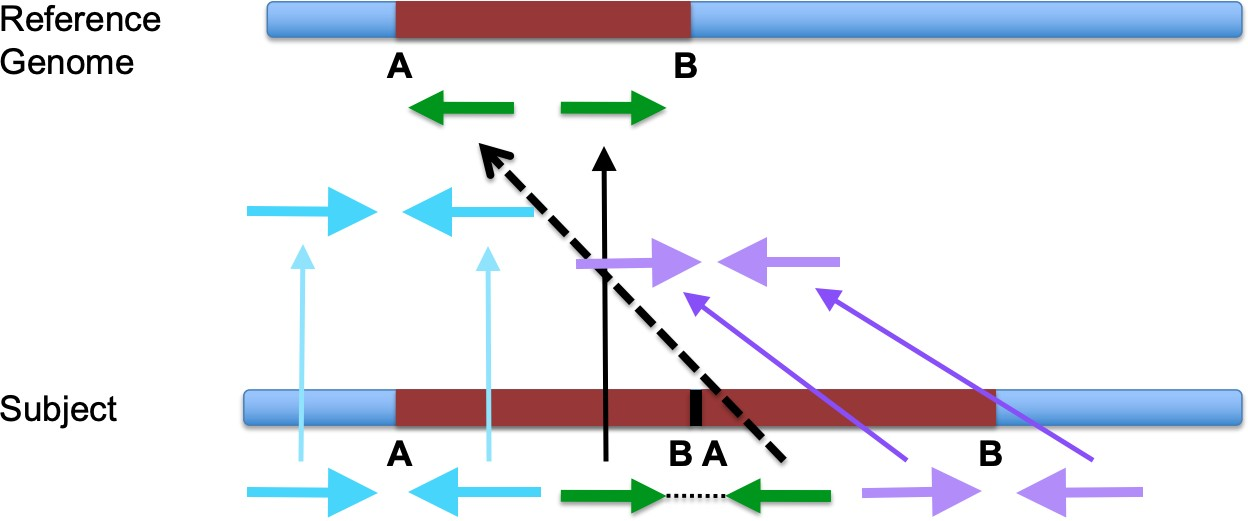
\includegraphics[width=6.1113in,height=2.55073in]{image23.jpeg}

\begin{quote}
So, as result, the orientation instead of going inward goes outward.

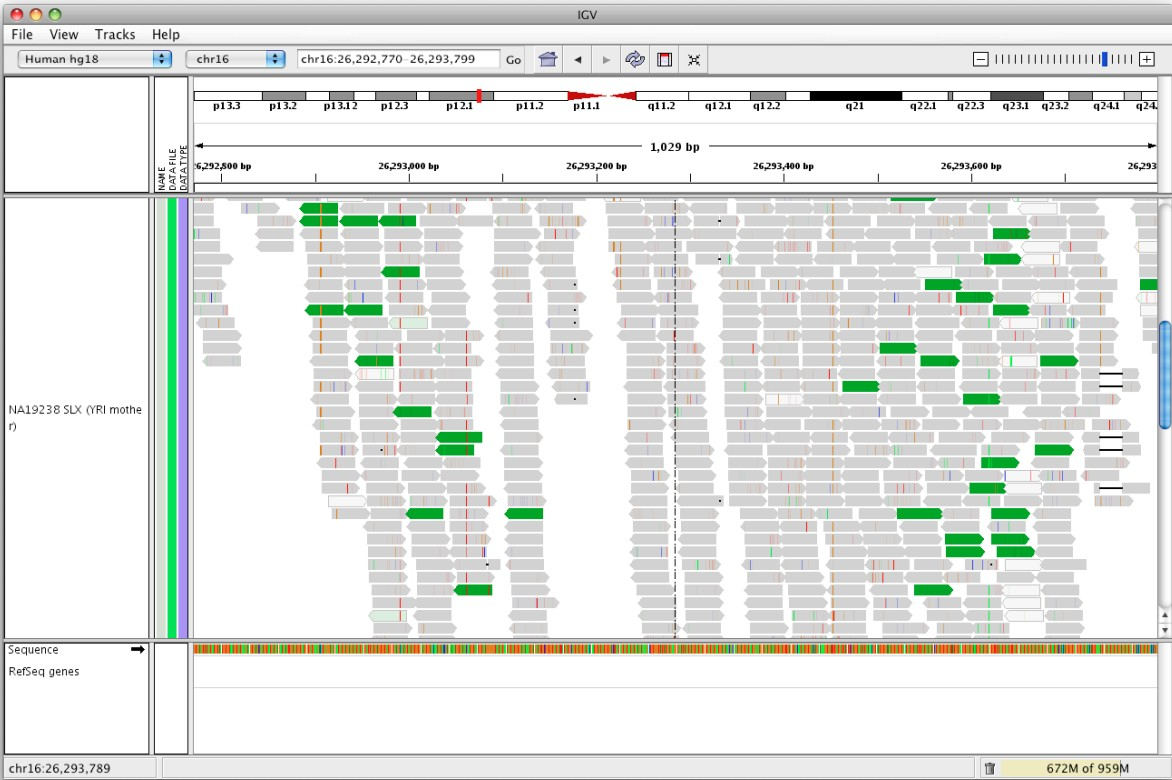
\includegraphics[width=6.22598in,height=4.14375in]{image24.jpeg}

\emph{What do you expect to see from coverage?} We will have a gain in
coverage that is proportional to the extra copy. We need to pay
attention to the double because it is a double contribution of that
allele, but if a tandem duplication happens only in one allele and the
other allele has his own one copy, then the local coverage corresponding
to the tandem duplication will be 3/2 of the expected coverage.

If you have a read that maps BA, do you expect to see it in the mapped
reads? Partial mapping. As we said before, if you allow your mapper to
have some mismatches of a certain percentage of bases from your reads,
you can still see some coverage contributed on one end of the segment
and mismatches on the other side.

For what concern the junctions, you shouldn't see any difference of
coverage because that sequence exists only once in the target molecule.
The local coverage increases only in correspondence of the segment AB.
\end{quote}

\hypertarget{inverted-duplication}{%
\subsection{Inverted duplication}\label{inverted-duplication}}

\begin{quote}
The duplication is inverted but it's not located near the original
fragment, but somewhere else

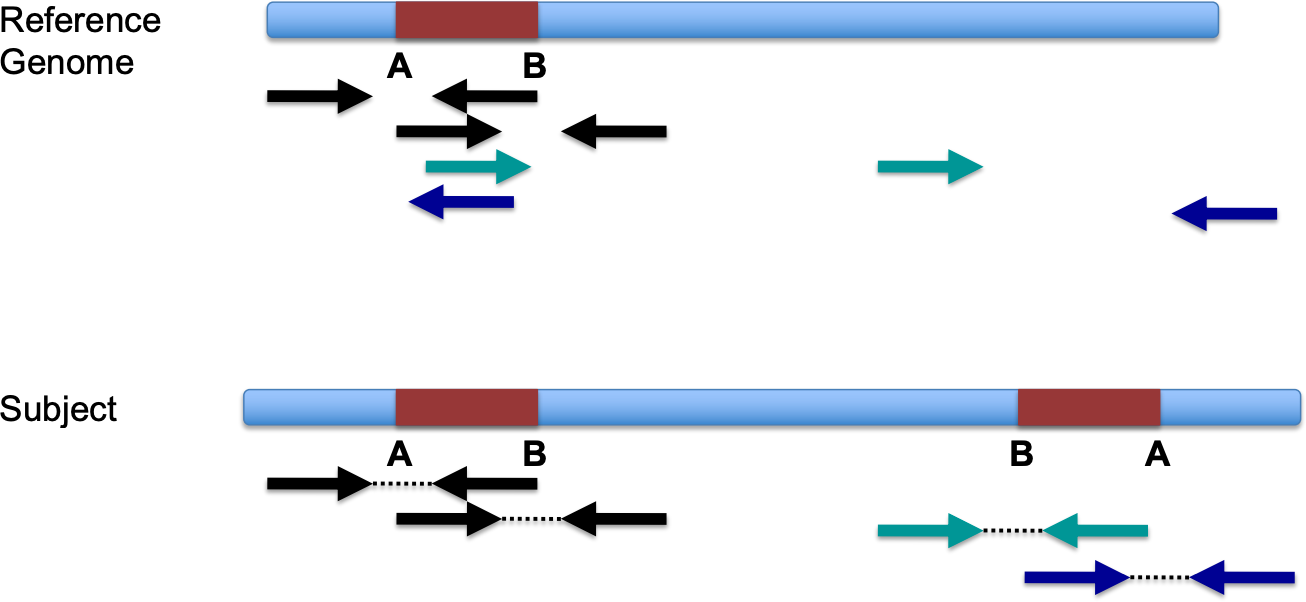
\includegraphics[width=6.11483in,height=2.82187in]{image25.png}

Take into consideration:
\end{quote}

\begin{itemize}
\item
  overlapping of ``left'' and ``right'' reads on the reference genome
\item
  coverage depth (copy number)
\end{itemize}

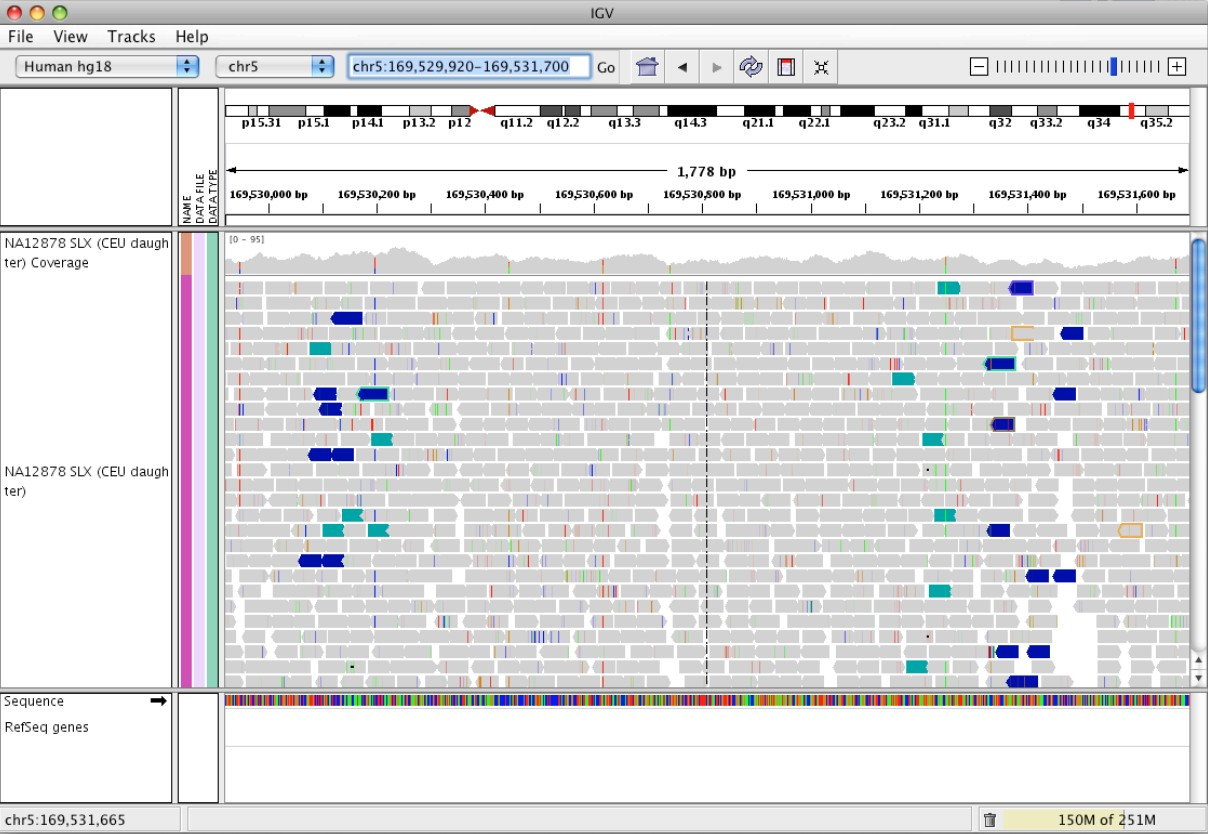
\includegraphics[width=6.29059in,height=4.34375in]{image26.jpeg}

\begin{quote}
There is a gain of coverage in the duplicated region and a tiny drop in
the break points where the sequence exists in only one allele
\end{quote}

\hypertarget{deletion}{%
\subsection{Deletion}\label{deletion}}

\begin{quote}
Deletion of a segment of DNA

If the deletion is larger than the size of the reads, we should see half
of the coverage in the deleted regions

If the deletion is larger that the size of the reads, we should see a
tiny little space corresponding to the missing nucleotides

Elements to consider:

Pair ends relative orientation Insert size length

Coverage within the aberrant region

Coverage outside of the aberrant region (flanking genomic segments)
Coverage at the breakpoints

Ask yourself if the sequence exists and where it is
\end{quote}
